% Desenho do sistema
\chapter{Desenho do sistema}
\label{cap3}

Os modelos propostos de interfaces com o utilizador, base de dados, classes e diagramas foram desenvolvidos no âmbito das disciplinas leccionadas até a data deste trabalho, reunindo assim neste trabalho todo um conjunto de aptidões e capacidades fundamentais para o desenvolvimento do sistema apresentado. Os pontos seguintes representam o trabalho desenvolvido e os métodos utilizados para o desenho do sistema.

\section{Modelação de interfaces}

Para o desenvolvimento das interfaces foram utilizados vários modelos, permitindo assim perceber de forma genérica as sequências de acções de navegação do utilizador. A figura \ref{fig:diagrama_arvore} representa uma árvore na qual podemos observar as páginas do portal e entender qual a ligação entre as diversas páginas utilizadas no portal.

\begin{figure}[!htb]
	\centering
	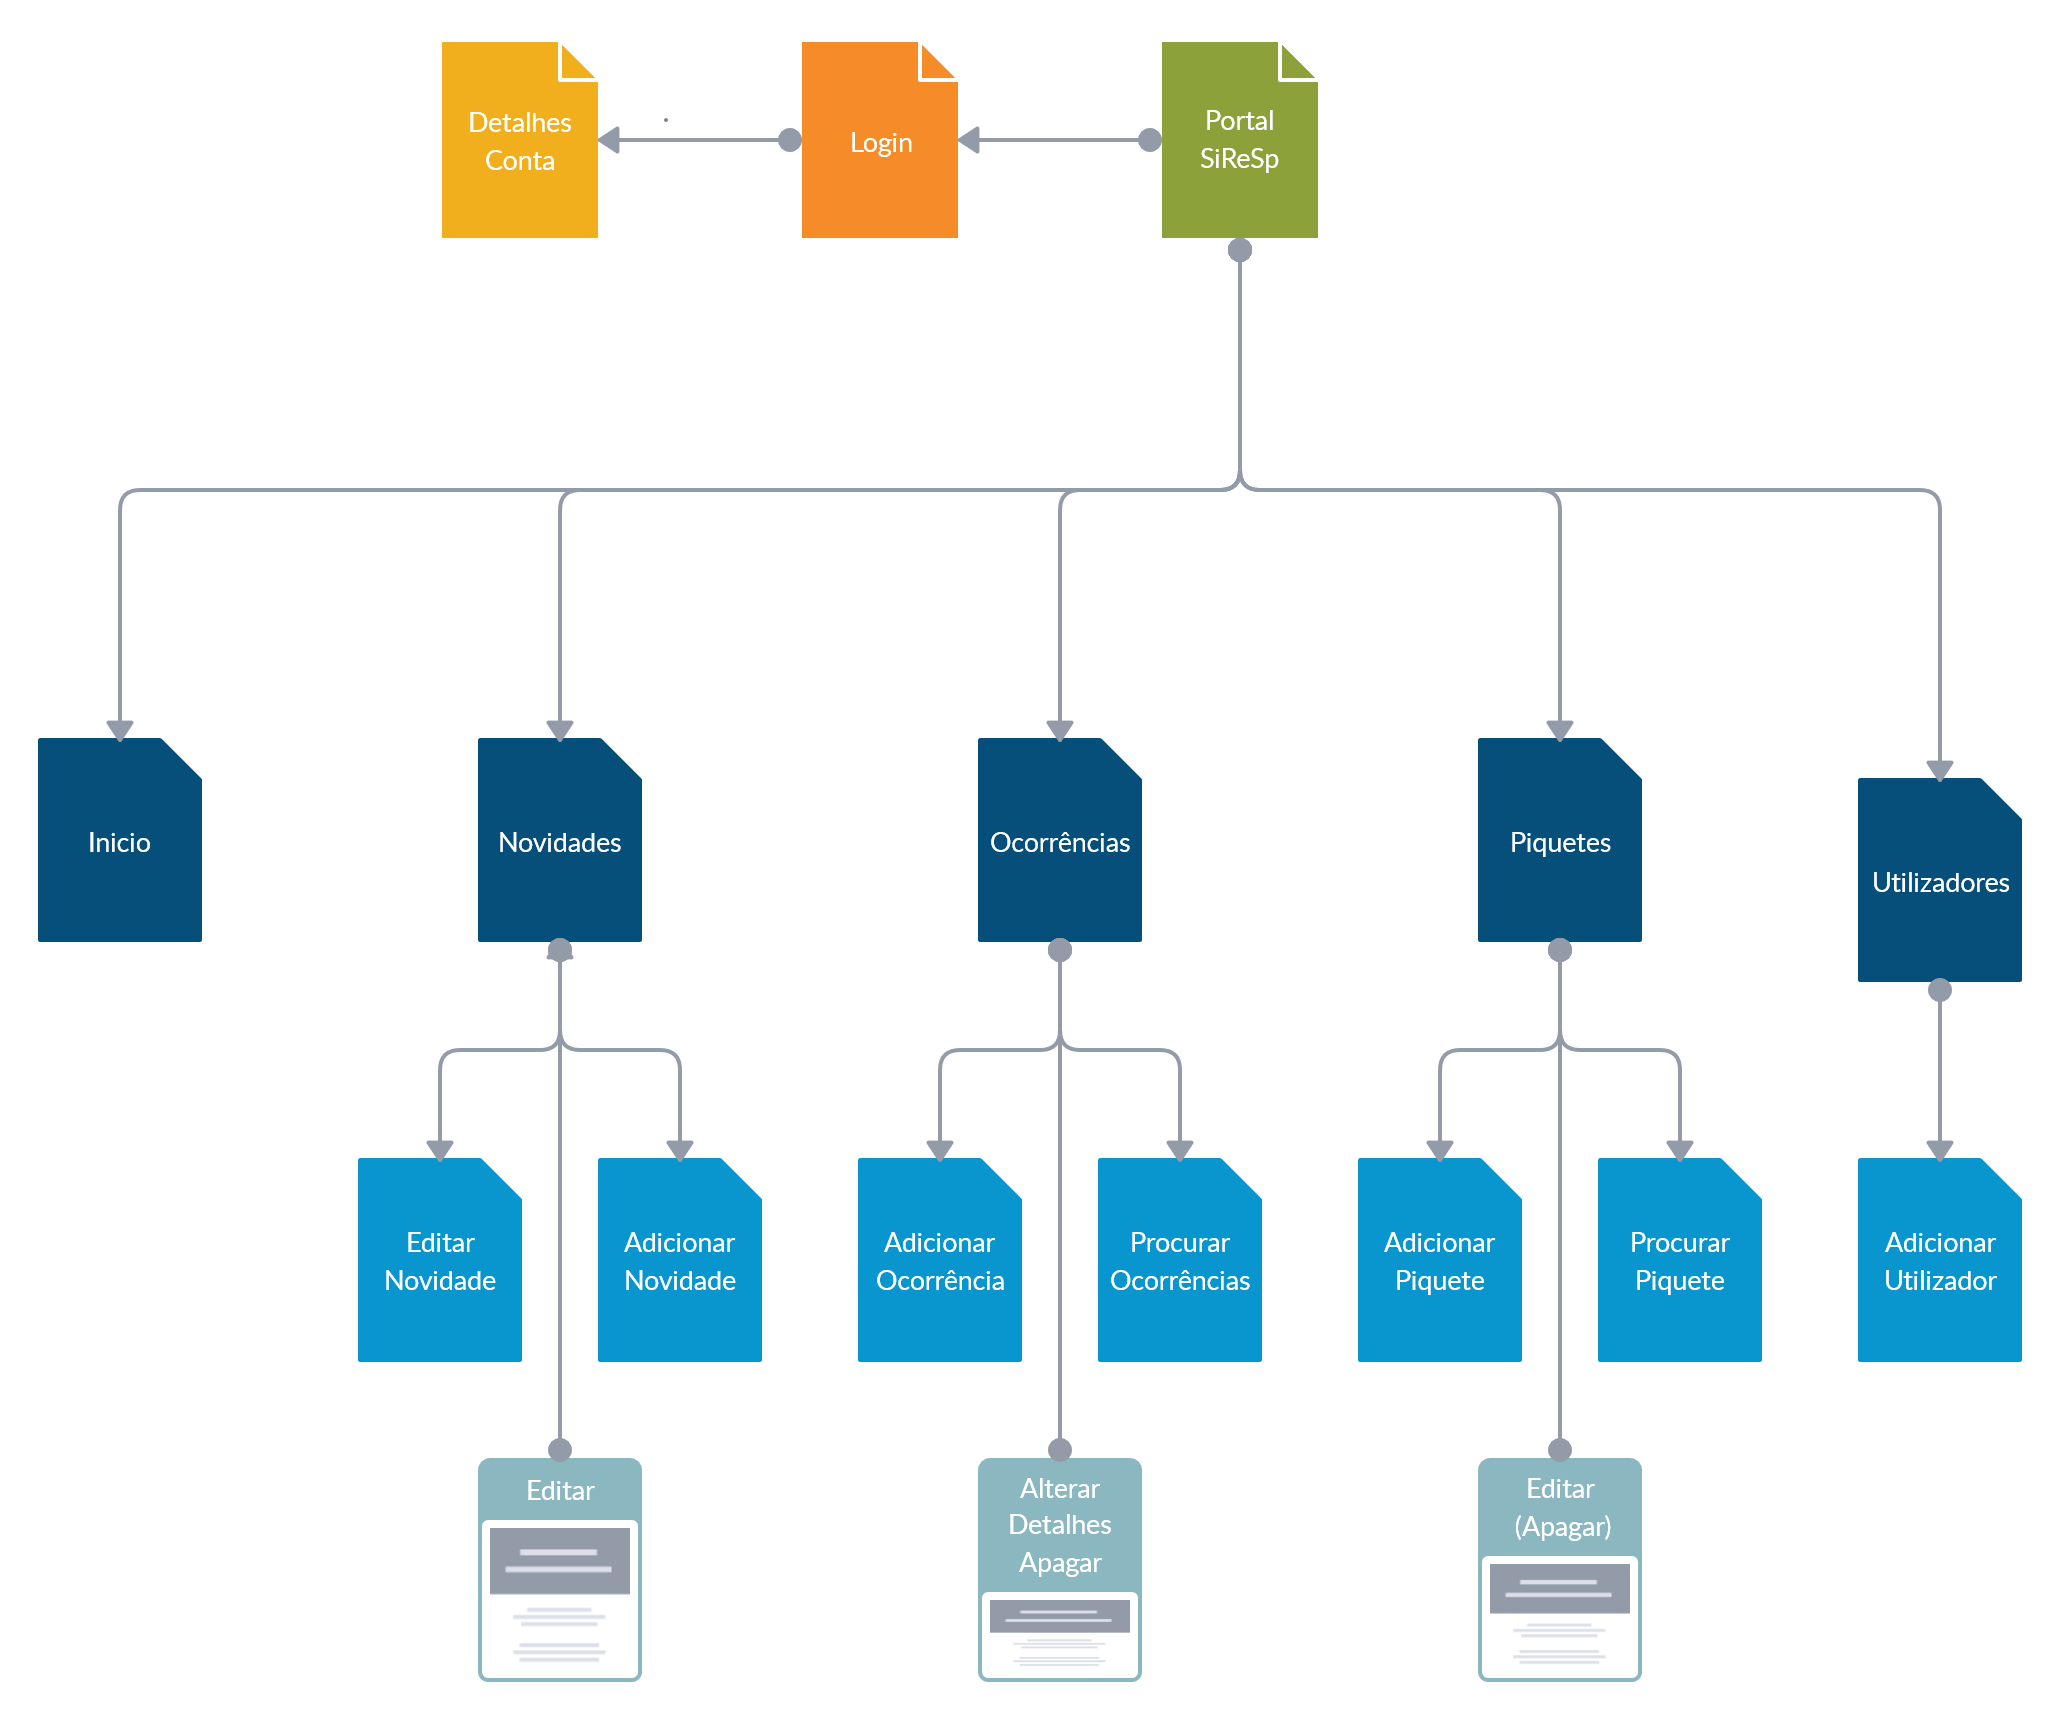
\includegraphics[width=\textwidth]{figuras/diagrama_arvore.png}
	\caption{Árvore de navegação no portal}
	\label{fig:diagrama_arvore}
\end{figure}

\subsection{Storyboard de navegação}

%Desenhos das paginas principais do frontend

\subsection{Interface do caso de uso 1}

%desenhos que descrevem a sequencia do casos de uso 1

\section{Modelação da base de dados}

A modelação da base de dados é fundamental para a implementação do sistema de forma correcta, o seu estudo e desenvolvimento são apresentados nos pontos seguintes e a forma como as entidades e classes estão relacionadas permite uma analise da complexidade do sistema, assim sendo, foi possível gerir a complexidade do modelo da base de dados de forma rigorosa. Em seguida são descritos os modelos E/R e físico da base de dados.

\subsection{Modelo Entidade-Relação}

A figura \ref{fig:Modelo_E/R} permite observar as relações entre as diversas entidades da base de dados. Através deste diagrama simplificado podemos visualizar as diversas acções que podem ser realizadas sobre o sistema.

\begin{figure}[!htb]
	\centering
	\includegraphics[width=\textwidth]{figuras/diagrama_e-r.png}
	\caption{Modelo entidade-relação}
	\label{fig:Modelo_E/R}
\end{figure}

\subsection{Modelo Físico}

O modelo físico, apresentado na figura \ref{fig:Modelo_fisico} complementa o modelo entidade-relação, especificando também os atributos de cada uma das tabelas.

\begin{figure}[!htb]
	\centering
	\includegraphics[width=\textwidth]{figuras/modelo_físico.png}
	\caption{Modelo físico}
	\label{fig:Modelo_fisico}
\end{figure}

\section{Modelação UML}



\subsection{Diagrama de classes}

modelo físico mais avançado

\begin{figure}[!htb]
	\centering
	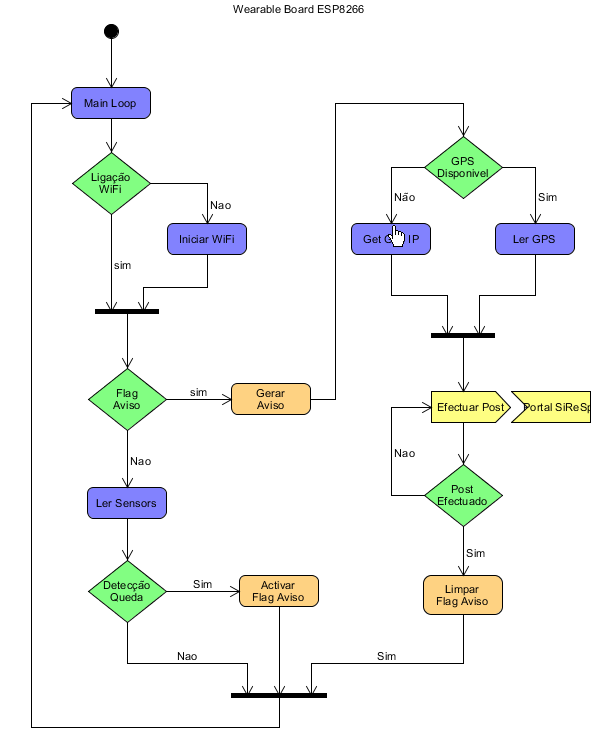
\includegraphics[width=\textwidth]{figuras/fluxograma_ESP.png}
	\caption{Fluxograma do funcionamento do ESP}
	\label{fig:fluxograma_ESP}
\end{figure}

\begin{figure}[!htb]
	\centering
	\includegraphics[width=\textwidth]{figuras/fluxograma_portal.png}
	\caption{Fluxograma do funcionamento do portal}
	\label{fig:fluxograma_portal}
\end{figure}

\subsection{Diagrama de sequência}

\subsection{Diagrama de sequência do caso de uso ...(ADICIONAR PIQUETE)}



\begin{figure}[!htb]
	\centering
	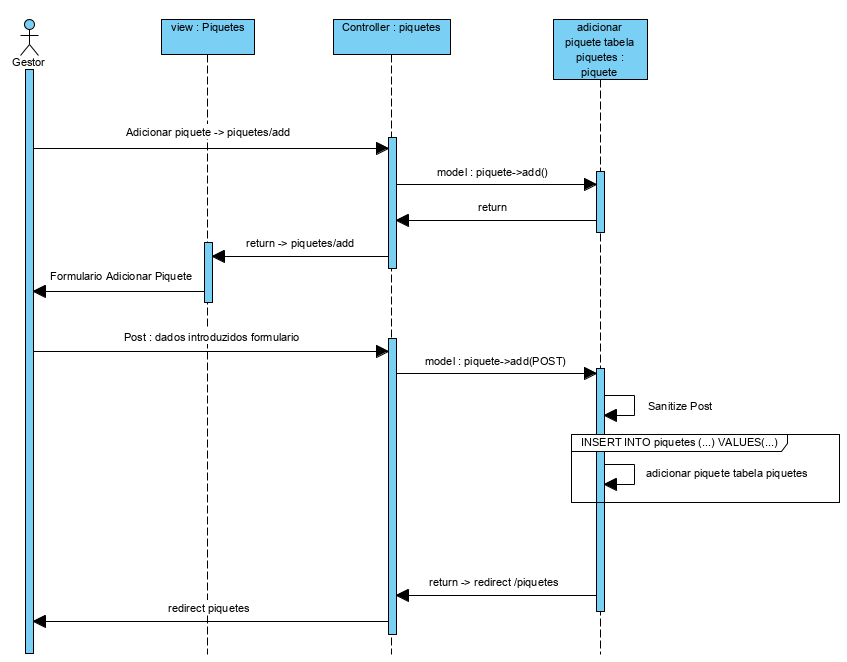
\includegraphics[width=\textwidth]{figuras/sequence_diagram_gestor.png}
	\caption{Diagrama de sequência para ...}
	\label{fig:sequência_gestor}
\end{figure}

\subsection{Diagrama de sequência do caso de uso ...(DETECÇÃO DE QUEDA)}



\begin{figure}[!htb]
	\centering
	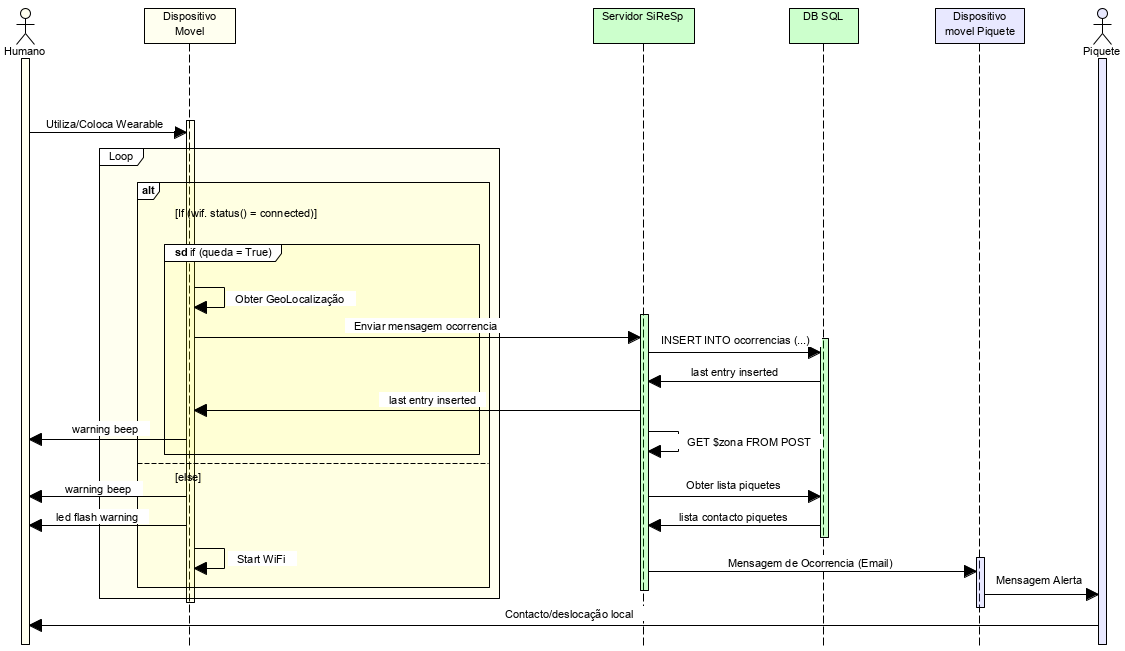
\includegraphics[width=\textwidth]{figuras/sequence_diagram_system_2.png}
	\caption{Diagrama de sequência para ...}
	\label{fig:sequência_sistema}
\end{figure}

\subsection{Diagrama de sequência do caso de uso ...(VISITANTE)}



\begin{figure}[!htb]
	\centering
	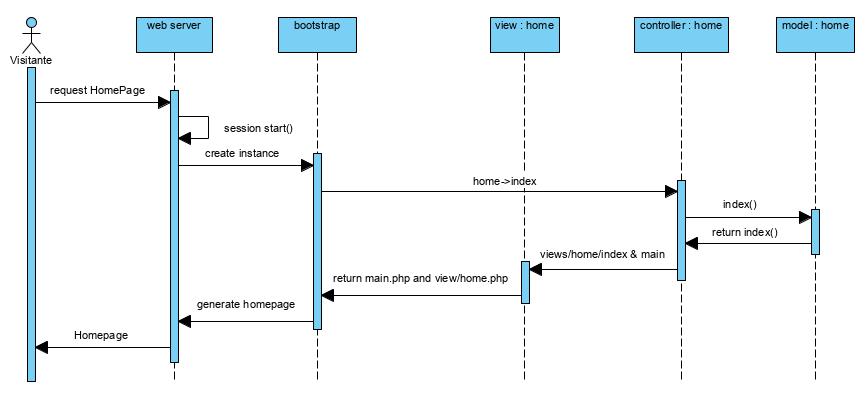
\includegraphics[width=\textwidth]{figuras/sequence_diagram_visitante.png}
	\caption{Diagrama de sequência para ...}
	\label{fig:sequência_visitamte}
\end{figure}